\section{Physical results}%
\label{sec:physicalresults}
In this section we report the results of the simulation.
We start discussing the lattice results for the correlation functions, along with their error and noise to signal ratio, then we present the energy gap $\DEt$
and the matrix element; finally, we show the continuum limit
extrapolations. The physical parameters $m$ and $\omega$ were both fixed at $1$ for every lattice and time $t$ is in units of the spacing $a$.
%In this section we show that we were able to numerically recover the physical results for the harmonic oscillator.
%Keeping the same parameters of table \ref{tab:A3} we will discuss the correlation functions and their error, then
%the discrete values of the energy gap $\DEt$ and matrix element $\matb$ and finally the continuum limit.
\subsection{Lattice results}%
\label{subsec:correlationfunctions}
Keeping a lattice with $N=256$ and $a=0.25$ as a case study, we computed the correlation functions $\ct$ (equation \ref{eqn:bestestim})
using $N_{bin}=10000$ bins of dimension $D_{bin}=500$.

Figures \ref{fig:corr} and \ref{fig:errcorr} show the correlators and their error.
\begin{figure}[h!]
\centering
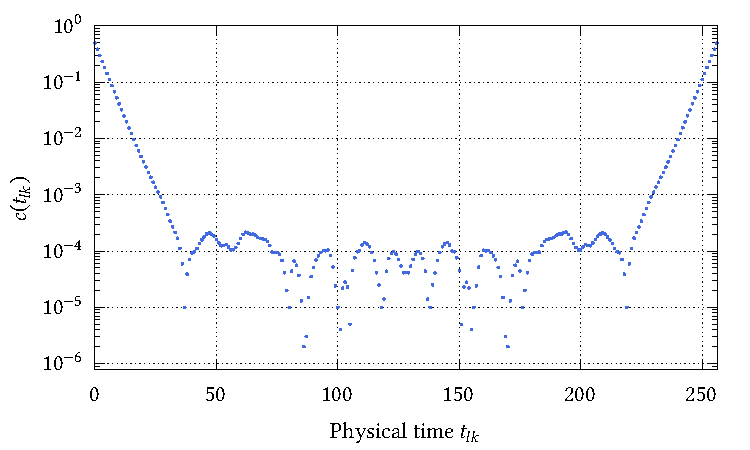
\includegraphics[width=\linewidth]{corr.pdf}
\caption{\label{fig:corr}Logarithmic plot of the correlators as a function of physical time. In this plot we highlight their symmetry with respect to $\t=128$,
more generally they are expected to be symmetric with respect to $\nicefrac{N}{2}$.}
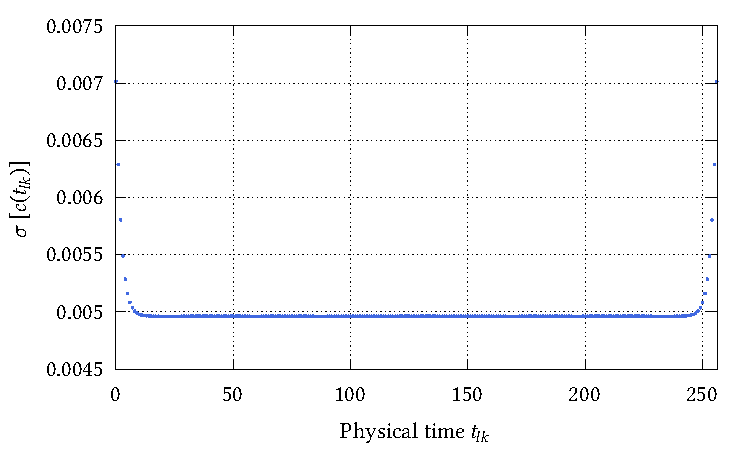
\includegraphics[width=\linewidth]{error}
\caption{\label{fig:errcorr}Standard error on the correlators. When $\lk$ is large, since $\ct$ is exponentially decreasing (equation \ref{eqn:correlators}), the error (equation \ref{eqn:bestvariance}) is dominated by
$\ev{x_{l}^{2}x_{k}^{2}}$ which is constant (equation \ref{eqn:xlxkq}).} 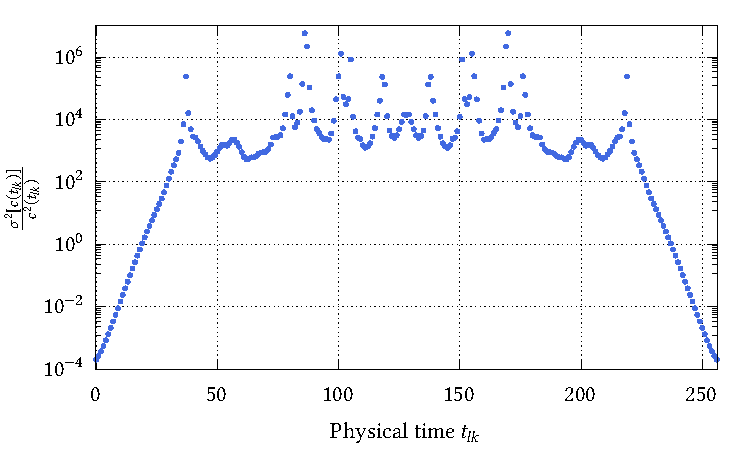
\includegraphics[width=\linewidth]{relerr.pdf}
  \caption{\label{fig:relerr}Logarithmic plot of the relative error squared. The exponential increase when $\lk$ grows but $\nicefrac{N}{2}\gg\lk$ is a manifestation of the so called exponential problem.}

\end{figure}
\\
We note that the plots demonstrate the expected features discussed in subsection \ref{subsec:purpose}: the correlators are symmetric with respect to the central site of the lattice (equation \ref{eqn:correlators}) and the error is constant when the distance between the lattice sites is large enough (equation \ref{eqn:varmatrix}).
Specifically, the errors cluster around $\sigma[\ct] = 0.004962$, which is the value we expect from the square root of equation \ref{eqn:varmatrix} for a lattice of spacing $a=0.25$ on which we considered $N_{bin}=10000$ configurations. Even though this is not enough to draw any definitive conclusions on $|\mel{\tilde{E_{0}}}{\x^{2}}{\tilde{E_{0}}}|$, as that would take a deeper analysis which is outside the scope of this experiment, we take it as a strong check of our results.
The symmetry allows us to discard correlators that depend on $\t > \nicefrac{N}{2}$ when computing $\DEt$ and $\matb$, as $c(\nicefrac{N}{2}+i)$ is identically equal to $c(\nicefrac{N}{2}-i)$ for any give site $i$.

Another expected feature, showcased by figure \ref{fig:relerr}, is the behaviour of the relative error. This is a manifestation of the exponential problem (equation \ref{eqn:relerr}) and will limit the number
of useful correlators in the following analysis.

\\

After computing the correlators $\ct$, we used them to calculate $\DEt$ (equation \ref{eqn:energy}) and $\matb$ (equation \ref{eqn:matelem}). This is when we had to consider two additional conditions: firstly, the observables are decorrelated on Markovian time but correlated on physical time; secondly, because of the exponential problem, as $\t$ grows so does the error, rendering later time calculations useless.

The physical time correlation is relevant because the energy gap, which is used itself to compute the matrix element,  is a
function of $\ct$, $\ctm$ and $\ctp$: we dealt with it applying the Jackknife method to resample the observables and automate the
statistical analysis for correlated variables. Regarding the exponential problem, we set a cutoff of $20\%$ to the relative error of each energy gap and matrix element value; only the surviving values were kept and used for the analysis.

In figure \ref{fig:energyA3} we show the $20$ surviving values of the energy and their error. Figure \ref{fig:matA3} does the same for the $15$ matrix elements.
%--------------------------------------
\begin{figure}[H]
  \centering
  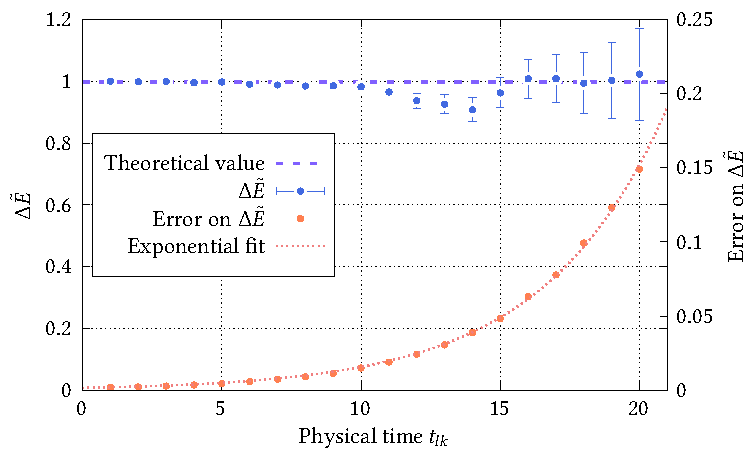
\includegraphics[width=\linewidth]{deltae}
  \caption{\label{fig:energyA3}In blue, energy gap from $\ct$ for different physical times; in orange, its error. The exponential growth of the error
  is highlighted.}
\end{figure}


\begin{figure}[H]
  \centering
  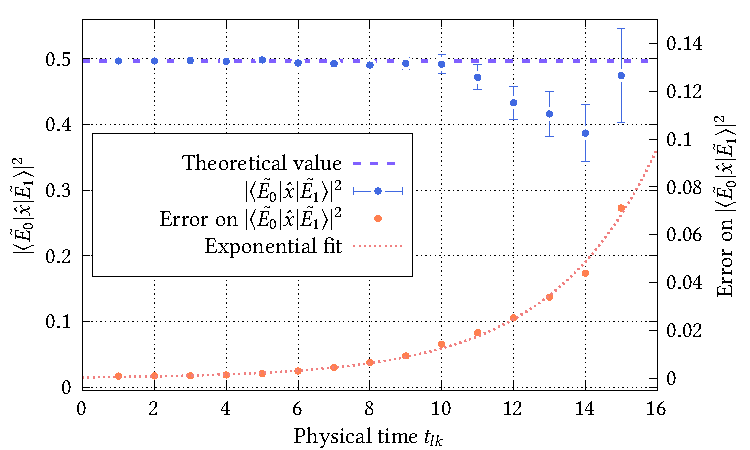
\includegraphics[width=\linewidth]{matelem}
  \caption{\label{fig:matA3} In blue, matrix element from $\ct$ for different physical times, the error bars are doubled to improve visibility; in orange, its error. The exponential growth of the error
  is highlighted.}
\end{figure}
%------------------------------------
The best estimates for $\DEt$ and $\matb$ are the weighted mean of the values that survive the cutoff and are collected in tables \ref{tab:energyresults} and \ref{tab:matrixresults}. The data shown in the figures correspond to the $A3$ lattice of table \ref{tab:alllattices}, which collects
the parameters of the five lattices that were used in the simulation.
% -----------------------------------------
\begin{table}[h!]
\centering
\begin{tabular}{@{}ccccc@{}}
\toprule
Lattice & $N$    & $a$      & $D_{bin}$ & $N_{bin}$ \\ \midrule
$A1$    & $64$   & $1$      & $50$      & $20000$   \\
$A2$    & $128$  & $0.5$    & $500$     & $10000$   \\
$A3$    & $256$  & $0.25$   & $500$     & $10000$   \\
$A4$    & $512$  & $0.125$  & $1000$    & $2000$    \\
$A5$    & $1024$ & $0.0625$ & $3000$    & $2000$    \\ \bottomrule
\end{tabular}
\caption{Parameters used for the different lattices.}
\label{tab:alllattices}
\end{table}
%---------------------------------------
\\
We kept the physical parameters $m=1$, $\w=1$, $Na=64$ fixed and repeated this procedure for each lattice of table \ref{tab:alllattices}. The more sites a lattice has, the higher the amount of values that survive the $20\%$ relative error cutoff: from lattice $A1$ to $A5$ we were able to work with a number of data in the order of $5$, $10$, $20$, $40$, $80$.
The results are collected in table \ref{tab:energyresults} for the energy gaps and table \ref{tab:matrixresults} for the matrix elements;
the theoretical values correspond to equation \ref{eqn:phys1} for $\DEt$ and equation \ref{eqn:phys2} for $\matb$.
%-------------------------------------------------------------------------------
\begin{table}[h!]
\centering
\begin{tabular}{@{}ccc@{}}
\toprule
Lattice              & \multicolumn{2}{c}{$\Delta\tilde{E}$} \\ \midrule
                     & Theoretical       & Obtained          \\
$A1$                 & $0.9624$          & $0.9634(17)$      \\
$A2$                 & $0.9899$          & $0.9887(13)$      \\
$A3$                 & $0.9974$          & $0.9970(11)$      \\
$A4$                 & $0.99935$         & $1.0002(6)$       \\
$A5$                 & $0.9998$          & $0.9993(5)$       \\ \bottomrule
\end{tabular}
 \caption{Energy gaps for the $5$ lattices.}
 \label{tab:energyresults}
\end{table}
%-----------------------------------------------------------------------------
\begin{table}[h!]
  \centering
\begin{tabular}{@{}ccc@{}}
\toprule
Lattice & \multicolumn{2}{c}{$\matb$}           \\ \midrule
                     & Theoretical       & Obtained          \\
$A1$                 & $0.4472$          & $0.4477(7)$       \\
$A2$                 & $0.4851$          & $0.4850(5)$       \\
$A3$                 & $0.4961$          & $0.4965(5)$       \\
$A4$                 & $0.4990$          & $0.4991(3)$       \\
$A5$                 & $0.4998$          & $0.4999(3)$       \\ \bottomrule
\end{tabular}
\caption{Matrix elements for the $5$ lattices.}
\label{tab:matrixresults}
\end{table}

\subsection{Continuum limit}%
\label{subsec:continuum limit}
We used the data gathered in tables \ref{tab:energyresults} and \ref{tab:matrixresults} to extract the physical properties of the continuum harmonic oscillator.
For both the energy gap and the matrix elements, according to equations \ref{eqn:fullen} and \ref{eqn:fullmat}, we performed a linear fit $y = m a ^2+q$ to find
$\Delta\tilde{E} = 0.9998(5)$ and $\matb = 0.4998(3)$ as the interception with the $y$ axis. The results are in good agreement with the theoretical values of $1$ and $0.5$.

Figures \ref{fig:contenergy} and \ref{fig:contmatelem} report the continuum limit for $\DEt$ and $\matb$ respectively, while figures \ref{fig:enerzoom} and \ref{fig:matzoom}
show close-ups of the points near the origin.

We also performed a \textit{full fit} those same equations to recover the frequency $\omega$ and the mass $m$ of the oscillator.
The results were satisfactory for the fit on $\DEt$, which had $\omega$ and $A$ as parameters
\begin{align}
  \DEt = \omega - \frac{\omega^{3}}{A}a^{2},
\end{align}
while the results for $\matb$ were less good. The model we used was
\begin{align}
  \matb = \frac{1}{2m\w}- \frac{\omega}{16 m}a^{2}
\end{align}
with $\w$ and $m$ as the fit parameters. Their values differ
from the expected ones by $8$ and $9$ standard deviations, but the correlation matrix suggests a very large negative correlation
between the fit parameters, which is not present in the theory
\begin{align}
  \label{eqn:cov}
  \crr =
  \begin{pmatrix}
    1 & -0.999\\
    -0.999 & 1\\
  \end{pmatrix}.
\end{align}

The results are collected in tables \ref{tab:entab} and \ref{tab:mattab}.
\begin{table}[h!]
  \centering
\begin{tabular}{@{}cccl@{}}
\toprule
\multicolumn{3}{c}{Linear fit}                 &           \\ \midrule
                   & Theoretical & Obtained    & $\sigma_{\text{s}}$ \\
$\Delta \tilde{E}$ & $1$         & $0.9998(5)$ & $0.4$     \\
Reduced $\chi^2$   & \multicolumn{3}{c}{$1.58$}            \\ \midrule
\multicolumn{3}{c}{Full fit}                   &           \\ \midrule
                   & Theoretical & Obtained    & $\sigma_{\text{s}}$ \\
$\omega$           & $1$         & $0.9998(5)$ & $0.4$     \\
$A$                & $24$        & $26.9(1.5)$ & $1.9$     \\
Reduced $\chi^2$   & \multicolumn{3}{c}{$1.58$}            \\ \bottomrule
\end{tabular}
\caption{\label{tab:entab}Continuum energy gap, frequency and $A$ parameter. All the results are inside a $2\sigma$ neighbourhood of their theoretical value. All the fits were performed by Gnuplot.}
\end{table}

\begin{table}[h!]
  \centering
\begin{tabular}{@{}cccl@{}}
\toprule
\multicolumn{3}{c}{Linear fit}               &           \\ \midrule
                 & Theoretical & Obtained    & $\sigma_{s}$ \\
$\matb$          & $0.5$       & $0.4998(3)$ & $0.67$    \\
Reduced $\chi^2$ & \multicolumn{3}{c}{$3.5$}             \\ \midrule
\multicolumn{3}{c}{Full fit}                 &           \\ \midrule
                 & Theoretical & Obtained    & $\sigma_{s}$ \\
$\omega$         & $1$         & $0.92(1)$   & $8$       \\
$m$              & $1$         & $1.09(1)$   & $9$       \\
Reduced $\chi^2$ & \multicolumn{3}{c}{$3.5$}             \\ \bottomrule
\end{tabular}
\caption{\label{tab:mattab} Results for the matrix element. The continuum limit is satisfactory, while the full fit returns incompatible results. The parameters extracted from the full fit also present a very high negative correlation (covariance matrix \ref{eqn:cov}), which could impact
the result of the fit. All the fits were performed by Gnuplot.}
\end{table}
%\onecolumn
%%------------------------ TABLE --------------------
\begin{table}[h!]
  \centering
\begin{tabular}{ccccccccc}
\hline
\multirow{2}{*}{} & \multirow{2}{*}{$N$} & \multirow{2}{*}{$a$} & \multirow{2}{*}{$D_{bin}$} & \multirow{2}{*}{$N_{bin}$} & \multicolumn{2}{c}{$\Delta\tilde{E}$}                            & \multicolumn{2}{c}{$\matb$}                                      \\ \cline{6-9}
           &       &                      &                            &                            & \multicolumn{1}{l}{Theoretical} & \multicolumn{1}{l}{Obtained} & \multicolumn{1}{l}{Theoretical} & \multicolumn{1}{l}{Obtained} \\ \hline
$A1$       &   $64$    & $1$                  & $50$                       & $20000$                    & $0.9624$                          & $0.9634(17)$                    & $0.4472$                         & $0.4477(7)$                   \\
$A2$       &   $128$   & $0.5$                & $500$                      & $10000$                    & $0.9899$                          & $0.9887(13)$                    & $0.4851$                         & $0.4850(5)$                   \\
$A3$       &   $256$    & $0.25$               & $500$                      & $10000$                    & $0.9974$                          & $0.9970(11)$                    & $0.4961$                         & $0.4965(5)$                   \\
$A4$       &   $512$    & $0.125$              & $1000$                     & $2000$                     & $0.99935$                          & $1.0002(6)$                    & $0.4990$                         & $0.4991(3)$                   \\
$A5$      &    $1024$    & $0.0625$             & $3000$                     & $2000$                      & $0.9998$                           & $0.9993(5)$                    & $0.4998$                         & $0.4999(3)$                  \\ \hline
\end{tabular}
\caption{\label{tab:bestvals}Summary of the lattices considered and their best values obtained for $\DEt$ and $\matb$.}
\end{table}
\twocolumn


%------------- FIGURES ------------
\begin{figure}[H]
  \centering
  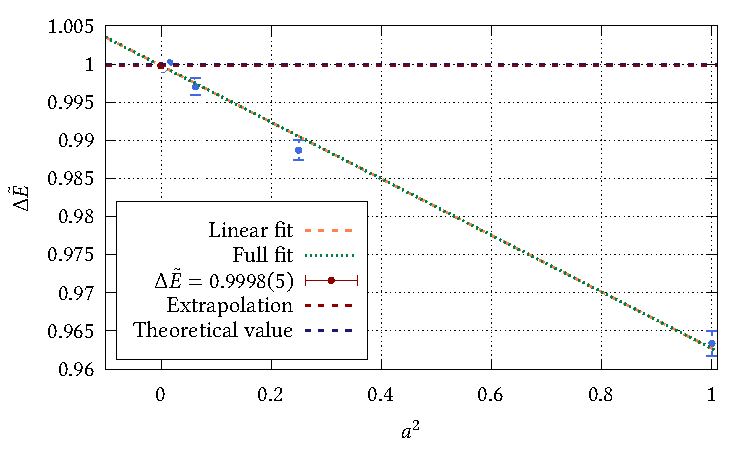
\includegraphics[width=\linewidth]{energy}
  \caption{\label{fig:contenergy}Energy gap continuum limit.}
\end{figure}
\begin{figure}[H]
  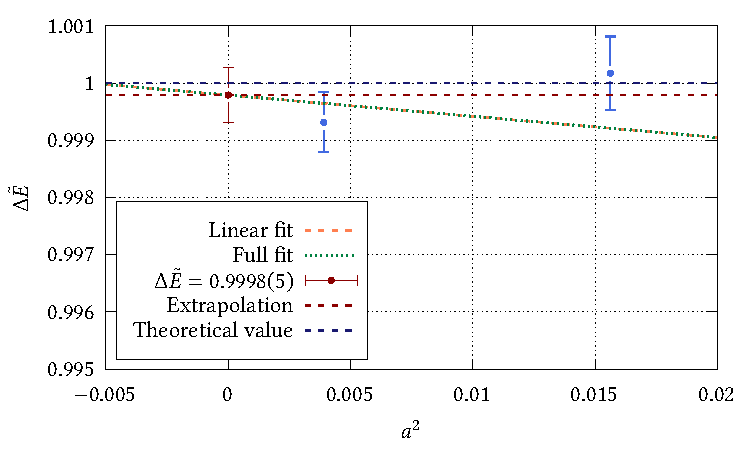
\includegraphics[width=\linewidth]{enerzoom}
  \caption{\label{fig:enerzoom}Close-up of the points next to the energy continuum limit.}
\end{figure}
\begin{figure}[H]
  \centering
  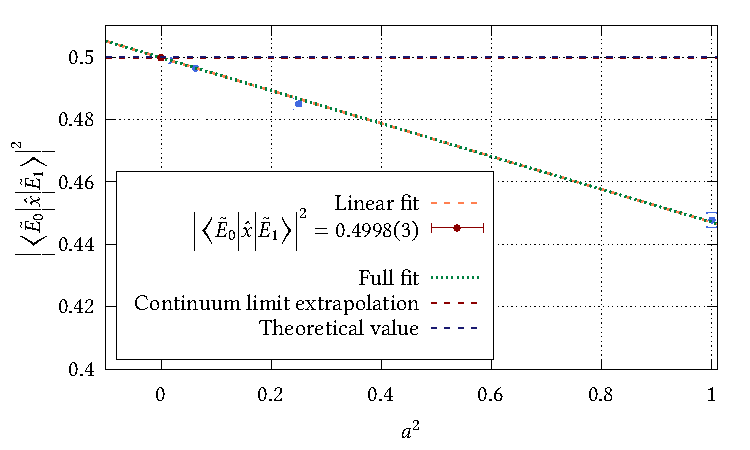
\includegraphics[width=\linewidth]{contmatelem}
  \caption{\label{fig:contmatelem}Matrix element continuum limit, error bars are doubled for visibility.}
\end{figure}
\begin{figure}[H]
  \centering
  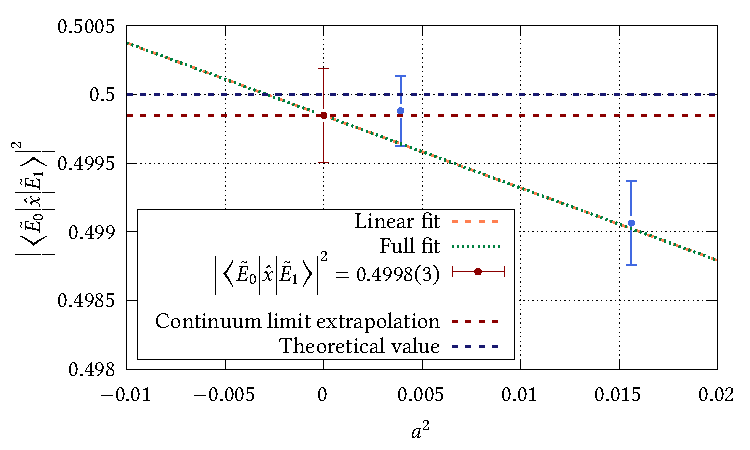
\includegraphics[width=\linewidth]{contmatelemtre}
  \caption{\label{fig:matzoom} Close-up of the points next to the matrix element continuum limit.}
\end{figure}


